\chapter{Portfolio Optimization}\label{portfolio-optimization}

Portfolio optimization models look for the optimal way to make investments. Usually investors expect either a maximum return for a given level of risk or a given return for a minimum risk so these models are typically based on two criteria: maximization of the expected return and/or minimization of the risk.

While the concept of return is straightforward there are a variety of risk measures. The most popular one has been variance in return and we will first look at it very closely before introducing some alternatives.

Some notations that will be used later are

\begin{itemize}
\tightlist
\item
  expected return: 
  \begin{equation} 
  	\mathbb{E}(R_{p}) = \sum _{i}w_{i} \mathbb{E}(R_{i}) 
  \end{equation} 
  where \(R_{p}\) is the return on the portfolio, \(R_{i}\) is the return on
  asset \(i\) and \(w_{i}\) is the weighting of component asset \(i\)
  (that is, the proportion of asset \(i\) in the portfolio) and
  \(\sum_{i}w_i = 1\) and \(0 \le w_i \le 1\);
\item
  portfolio return variance:
  \begin{equation} 
 	\sigma _{p}^{2} = \sum _{i}w_{i}^{2}\sigma _{i}^{2} + \sum _{i}\sum _{j\neq i}w_{i}w_{j}\sigma _{i}\sigma _{j}\rho _{ij} \end{equation}
  where \(\sigma\) is the (sample) standard deviation of the periodic
  returns on an asset, and \(\rho _{ij}\) is the correlation coefficient
  between the returns on assets \(i\) and \(j\). In a more compact way
  it can be expressed as:
  \begin{equation} 
  	\sigma _{p}^{2}=\sum _{i}\sum _{j}w_{i}w_{j}\sigma _{ij} 
  \end{equation} 
  where \(\sigma _{ij}=\sigma _{i}\sigma _{j}\rho _{ij}\) is the (sample)
  covariance of the periodic returns on the two assets, or alternatively
  denoted as \(\Sigma\).
  In matrix notation:
  \begin{equation}
  	\sigma_p^2 = \mathbf{w^T}\Sigma\mathbf{w} 
  \end{equation}
  where $\mathbf{w} = (w_1,w_2,\ldots,w_N)$ is the vector of weights. 
  For a very brief introduction to matrices see Appendix~\ref{app:matrices};
\item
  portfolio return volatility (standard deviation):
  \begin{equation}
  	\sigma _{p}= \sqrt{\sigma _{p}^{2}}
  \end{equation}
\end{itemize}

\section{The Markowitz Mean/Variance Portfolio Model}
\label{the-markowitz-meanvariance-portfolio-model}

Although investors may expect a particular return when they buy a stock, they may be disappointed or pleasantly surprised, because fluctuations in stock prices result in fluctuating returns. 

This model, first introduced by Markowitz, defines risk as the possibility that actual returns will deviate from expected returns, and the degree of potential fluctuation determines the degree of risk.
So it assumes that an investor has two considerations when constructing an investment portfolio: expected return and variance in return (i.e. measure of risk or of the variability in realized return around the expected return). 

Hence the Markowitz model requires two major kinds of information:

\begin{itemize}
\tightlist
\item
  the estimated expected return for each candidate investment;
\item
  the covariance matrix of returns, which characterizes not only the 
  individual variability of the return on each investment, 
  but also how each investment's return tends to move with the other (correlation).
\end{itemize}

In the following examples we are going to use real data
of five companies:  AAPL, AMZN, FB, GOOG, NFLX. As for data used in the previous Chapter
it can be downloaded with \texttt{ffn}:

\begin{ipython}
import pandas as pd
import ffn

df = ffn.get('aapl,AMZN,FB,GOOG,NFLX', start='2014-03-27', end='2018-03-27')
# uncomment the following line if reading from file
# df = pd.read_csv("portfolio_data.csv", index_col="date")

print (df.head())
\end{ipython}
\begin{ioutput}
                aapl       amzn        fb       goog      nflx
Date
2014-03-27 17.202097 338.470001 60.970001 556.930969 52.025715
2014-03-28 17.182892 338.290009	60.009998 558.456787 51.267143
2014-03-31 17.179056 336.369995	60.240002 555.445007 50.290001
2014-04-01 17.336205 342.989990	62.619999 565.607117 52.098572
2014-04-02 17.365013 341.959991	62.720001 565.447571 51.840000
\end{ioutput}

Otherwise it can be directly used from \href{https://raw.githubusercontent.com/matteosan1/finance_course/develop/libro/input_files/portfolio_data.csv}{portfolio\_data.csv}. 
Data, shown in Figure~\ref{fig:stocks}, is made of the historical 
series of the closing prices in the last 5 years. 

With \texttt{pandas} the main characteristics of these time series can
be easily computed (e.g. daily returns, covariance matrix,\ldots):

\begin{ipython}
daily_returns = df.pct_change()
returns = daily_returns.mean()*252
print (returns)
\end{ipython}
\begin{ioutput}
aapl    0.240921
amzn    0.414775
fb      0.263708
goog    0.173464
nflx    0.527628
dtype: float64
\end{ioutput}

\begin{ipython}
covariance = daily_returns.cov()*252
print (covariance)
\end{ipython}
\begin{ioutput}
          aapl      amzn        fb      goog      nflx
aapl  0.051967  0.025182  0.026075  0.022764  0.028064
amzn  0.025182  0.085876  0.041196  0.039654  0.048576
fb    0.026075  0.041196  0.069723  0.036337  0.044753
goog  0.022764  0.039654  0.036337  0.052001  0.040630
nflx  0.028064  0.048576  0.044753  0.040630  0.178332
\end{ioutput}

\begin{figure}[htb]
\centering
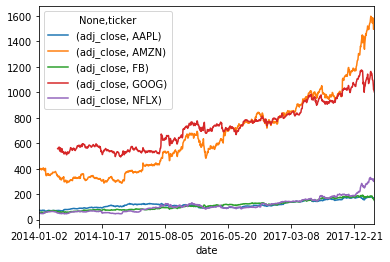
\includegraphics[width=0.7\textwidth]{figures/portfolio_sample}
\caption{Historical series of the closing price of five companies. To compare them, prices, have been normalized to the 
first value in each series}
\label{fig:stocks}
\end{figure}
    
In order to "simulate" a portfolio it is enough to throw five random weights with the constraint that they had to sum up to 1. 
In Figure~\ref{fig:mc_portfolio} a large number of simulated portfolios are shown in the return vs volatility plane. 
In this case no attempt of any optimization whatsoever has been made.

\begin{figure}[hbt]
\centering
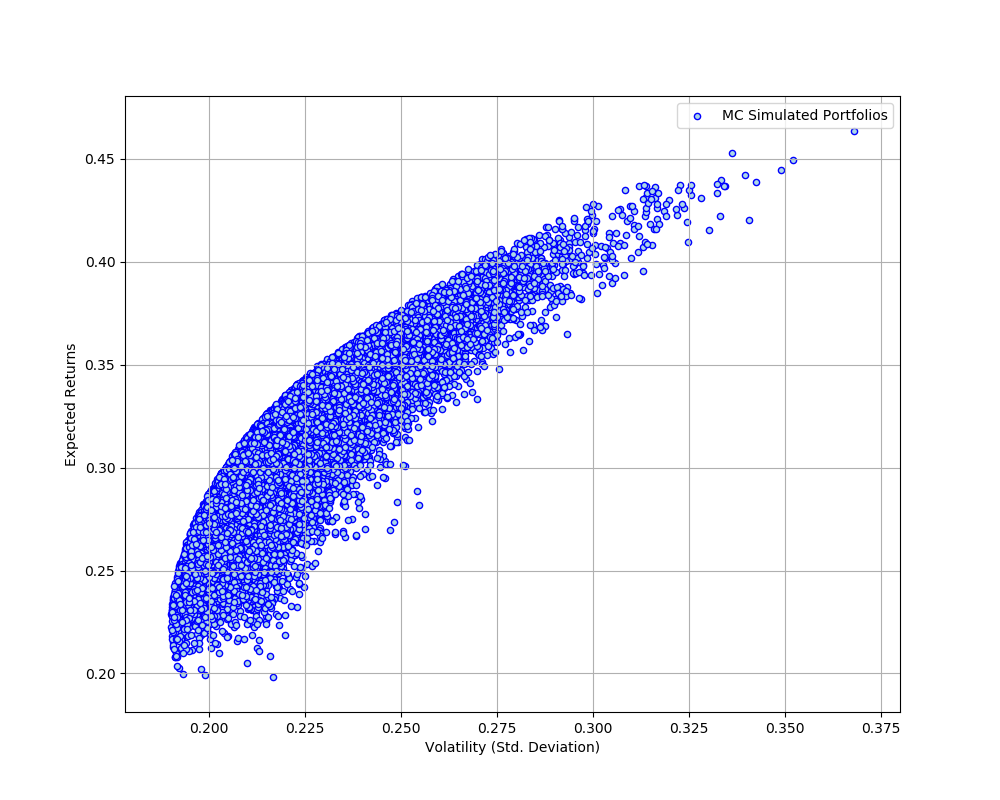
\includegraphics[width=0.8\textwidth]{figures/return_variance}
\caption{Distribution in the expected return/volatility plane of a large number of simulated portfolios.}
\label{fig:mc_portfolio}
\end{figure}

Investors may use short sales in their portfolios (a portfolio is short in those stocks with negative portfolio weights). 
Although short selling extends the set of possible portfolios we are not going to consider them here.

\section{Optimisation}\label{optimization}

Markowitz model states that \emph{the weights of a portfolio should be chosen 
such that its volatility (or its variance) is minimised}. 
So the application of this model reduces to
an optimisation problem: given the covariance matrix of the portfolio
$\Sigma$, estimated from their historical series, we need to find

\begin{equation}
	\underset{\mathbf{w}}{\min}\{\sigma_p^2\} = \underset{\mathbf{w}}{\min}\{\mathbf{w^T}\Sigma\mathbf{w}\}
\end{equation}
with the constraints \(\sum_{i}w_i = 1\) and \(0 \le w_i \le 1\).

In \texttt{python} we already know how to solve a minimisation problem
(see bootstrapping in Chapter~\ref{sec:swaps-and-bootstrapping}) 
so it is enough to repeat the same steps:

\begin{itemize}
\tightlist
\item
  define an objective function (in this case the portfolio variance);
\item
  define a set of constraints ($\sum w_i = 1$);
\item
  set an initial guess for the weights;
\item
  pass everything to \texttt{scipy.optimize.minimize}.
\end{itemize}

\begin{ipython}
import numpy as np
from scipy.optimize import minimize

def sum_weights(w):
    return np.*@sum@*(w) - 1

def markowitz(w, cov):
    return w.T.dot(cov.dot(w))

num_assets = 5
constraints = ({'type': 'eq', 'fun': sum_weights},)
bounds = tuple((0, 1) for asset in range(num_assets))
weights = [1./num_assets for _ in range(num_assets)]
opts = minimize(markowitz, weights, args=(covariance,),
                bounds=bounds, constraints=constraints)
print (opts)
print ("Expected portfolio return: {:.3f}".format(np.dot(opts.x, returns))
\end{ipython}
\begin{ioutput}
    fun: 0.036290306589982405
    jac: array([0.07274766, 0.07278468, 0.07233336, 0.07242217, 0.0726624 ])
message: 'Optimization terminated successfully.'
   nfev: 63
    nit: 9
   njev: 9
 status: 0
success: True
x: array([0.44644822, 0.06472903, 0.12215803, 0.36453326, 0.00213147])

Expected portfolio return: 0.231
\end{ioutput}

The solution recommends to devote about 44\% of the portfolio to AAPL, about 6\% to AMZN, 12\% to FB and so on\ldots The expected return is about 23\%, with a variance of about 0.036 or, equivalently, a standard deviation of 0.19.

In this example we based the model simply on straightforward statistical data derived from daily returns. However it could be possible, rather than estimate the expected returns from historical data, to base this estimate on information about expected future performance of the asset.

\section{Efficient Frontier}\label{efficient-frontier}
There is no precise way for an investor to determine the “correct” trade off between risk and return. If she wants a higher expected return, she generally has to “pay for it” with higher risk. Thus, one is frequently interested in looking at the relative distribution of the two.

In finance terminology, we would like to trace out the \emph{efficient frontier} of return and risk. This is doable solving for the minimum variance portfolio over a range of values for the expected return (e.g. ranging from 0.20 to 0.45).

This time beside the constraint on the sum of weights, we have to add the one that forces the resulting return to be equal to the chosen target.

The following example produce the efficient frontier plot shown in Fig.~\ref{fig:efficient_frontier}.

\begin{ipython}
def efficient_frontier(w, asset_returns, target_return):
    portfolio_return = asset_returns.dot(w)
    return (portfolio_return - target_return)

results = []
bounds = tuple((0, 1) for asset in range(num_assets))
for eff in np.arange(0.20, 0.45, 0.005):
    constraints = ({'type': 'eq', 'fun': efficient_frontier,
                    'args':(returns, eff,)},
                   {'type': 'eq', 'fun': sum_weights})
weights = [1./num_assets for _ in range(num_assets)]
opts = minimize(markowitz, weights, args=(covariance,),
                bounds=bounds, constraints=constraints)
results.append((np.sqrt(opts.x.T.dot(covariance.dot(opts.x))),
                np.*@sum@*(returns*opts.x)))
\end{ipython}

\begin{figure}[htb]
\centering
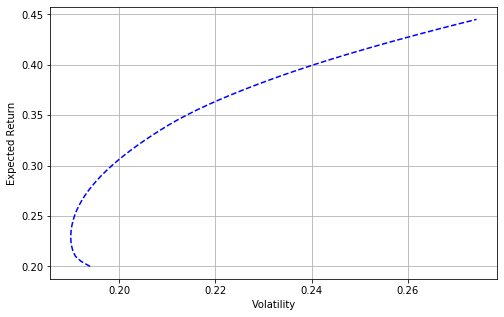
\includegraphics[width=0.7\textwidth]{figures/efficient_frontier.png}
\caption{Efficient frontier for our example portfolio obtained minimizing the the variance and requiring an expected return between 0.02 and 0.45.}
\label{fig:efficient_frontier}
\end{figure}

Efficient portfolios offer investors the highest possible expected return for a given level of risk. 
An investor seeking high expected returns and low volatility should invest only in efficient portfolios and will choose from the set of efficient portfolios based on her risk tolerance.
    
\subsection{Limits of the Markowitz Model}
\label{limits-of-the-markowitz-model}
    
Despite the significant utility of the Markowitz theory, there are some major limitations in this model:
    
\begin{itemize}
  	\tightlist
   	\item
   	it is difficult to forecast asset returns with accuracy using
   	historical data, which tends to be a poor forecasting source. As
   	return estimates have a much larger impact on the asset allocations,
   	small changes in return assumptions can lead to inefficient
   	portfolios. Therefore, the model tends to lead to highly concentrated
   	portfolios (out-of sample weights) that do not offer as much
   	diversification benefits in practice as they seem to provide in
   	theory;
   	\item
    the correlation between assets is assumed to be fixed and predictable, while
    in the real world, the systematic relationships between different assets 
    do not remain constant. This means that the theory becomes less useful during 
    times of uncertainty, which is exactly when investors need the most protection 
    from volatility.
    \end{itemize}
    
Extensions of the Markowitz model are defined in~\cite{bib:post_modern_theory} and~\cite{bib:black_litterman}, 
although they are beyond the scope of these lectures. 
    
\section{Portfolios with a Risk-Free Asset}
\label{portfolios-with-a-risk-free-asset}

When one of the investments available is risk free, then the efficient frontier has a particularly simple form. The risk–return combinations of the risk-free investment and a risky portfolio lie on a straight line connecting the two investments: the capital allocation line (CAL). The slope of the CAL measures the trade off between risk and return. A higher slope means that investors receive a higher expected return in exchange for taking on more risk.

The capital allocation line aids investors in choosing how much to invest in a risk-free asset and one or more risky assets.

The simplest example of such kind of portfolios is the one containing only two assets: a risk-free Treasury bill and a stock. Assume that the expected return of the Treasury bill is \(\mathbb{E}(R_f)=3\%\) and its risk is 0\%. Further, assume that the expected return of the stock is \(\mathbb{E}(R_r)=10\%\) and its standard deviation is \(\sigma_r=20\%\). The question that needs to be answered for any individual investor is how much to invest in each of these
assets.

The expected return (\(\mathbb{E}(R_p)\)) of this portfolio is calculated as follows:

\begin{equation*} 
	\mathbb{E}(R_p) = \mathbb{E}(R_f)\cdot w_f + \mathbb{E}(R_r)\cdot (1- w_f) 
\end{equation*}
where \(w_f\) is the relative allocation to the risk-free asset.

The calculation of risk for this portfolio is simple because the standard deviation of the Treasury bill is 0\%. Thus it is calculated as

\begin{equation*} 
	\sigma_p = (1-w_f)\cdot \sigma_r 
\end{equation*}
In this very simple example, if an investor invested 100\% into the risk-free asset (\(w_f=1\)), the expected return would be 3\% and the risk of the portfolio would be 0\%. Likewise, investing 100\% into the stock (\(w_f=0\)) would give an investor an expected return of 10\% and a portfolio risk of 20\%. If the investor allocated 25\% to the risk-free asset and 75\% to the risky asset, the portfolio expected return and risk calculations would be

\[ \mathbb{E}(R_p) = (3\% \cdot 25\%) + (10\% \cdot 75\%) = 0.75\% + 7.5\% = 8.25\% \]

\[ \sigma_p = 75\% \cdot 20\% = 15\% \]

Applying the same reasoning to our example we can consider an additional risk-free asset with an expected return of 10\% and repeat the minimisation to determine the efficient frontier of the resulting portfolio. Notice how the objective function is almost the same as before, while the target return constraint now includes the risk-free asset.

\begin{ipython}
num_assets = 6

def markowitz_with_rf(w, cov):
    return w[:-1].T.dot(cov.dot(w[:-1]))

def efficient_frontier_with_rf(w, asset_returns, target_return, risk_free):
    portfolio_return = np.*@sum@*(asset_returns*w[:-1]) + risk_free*w[5]
    return (portfolio_return - target_return)

rf_asset_return = 0.10
res_rf = []
bounds = tuple((0, 1) for asset in range(num_assets))
for eff in np.arange(0.10, 0.45, 0.01):
    constraints = ({'type': 'eq', 'fun': efficient_frontier_with_rf,
	                'args':(returns, eff, rf_asset_return)},
                   {'type': 'eq', 'fun': sum_weights})
    weights = [1./num_assets for _ in range(num_assets)]
    opts = minimize(markowitz_with_rf, weights, args=(covariance),
                    bounds=bounds, constraints=constraints)
    res_rf.append((np.sqrt(opts.x[:-1].T.dot(covariance.dot(opts.x[:-1]))),
                   np.*@sum@*(returns*opts.x[:-1])+opts.x[5]*rf_asset_return))
\end{ipython}

\begin{figure}[htb]
\centering
    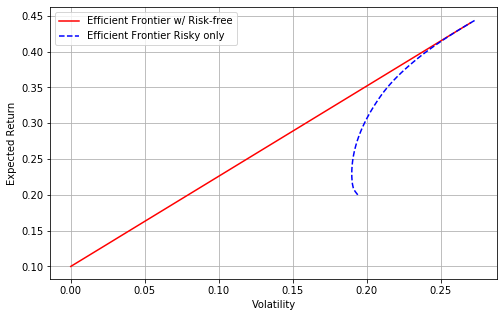
\includegraphics[width=0.7\textwidth]{figures/cal.png}
    \caption{Comparison of efficient frontier with a risk-free asset (red) and with risky asset only (blue).}
    \label{fig:cal}
\end{figure}
    
As it is clear from Fig.~\ref{fig:cal} the efficient frontier has become a straight line, tangent to the frontier of the risky assets only. When the target is 10\% the entire investment is allocated to the risk-free asset, as the target increases the fraction of the risky assets grows
proportionally to the volatility. 

It is important to notice that in general the relative proportions devoted to risky investments do not change. Only the allocation between the risk-free asset and the risky assets change.

\subsection{The Sharpe Ratio}
\label{the-sharpe-ratio}
The goal of an investor who is seeking to earn the highest possible expected return for any level of volatility is to find the portfolio that generates the steepest possible line when combined with the risk-free investment. The slope of the line is called the \emph{Sharpe ratio} of the portfolio.

For some portfolio of risky assets let 

\begin{itemize}
\tightlist
\item
  \(R_r\) its expected return;
\item
  \(\sigma_r\) its standard deviation in return;
\item
  \(r_f\) the return of a risk-free asset.
\end{itemize}

A plausible single measure (as opposed to the two measures, risk and return) of attractiveness of portfolio is the Sharpe ratio:

\begin{equation} \cfrac{R_r - r_f}{\sigma_r} \end{equation}

In words, it measures how much additional return we achieved for the additional risk we took on, relative to putting all our money in the risk-free asset. The portfolio that maximizes this ratio has some interesting properties. Suppose 

\begin{itemize}
\tightlist
\item
  \(R_\textrm{target}\) our desired target return;
\item
  \(w_r\) the fraction of our wealth we place in the portfolio (the
  rest placed in the risk-free asset).
\end{itemize}

To meet our return target, we must have:

\begin{equation*} 
	(1 - w_r) * r_f + w_r * R_r =R_\textrm{target} 
\end{equation*}

The standard deviation of our total investment is: \(w_r\cdot \sigma_r\). Solving for \(w_r\) in the equation above, we get:

\begin{equation*} 
	w_r = \cfrac{R_\textrm{target} - r_f}{R_r - r_f} 
\end{equation*}
Thus, the standard deviation of the portfolio is:

\begin{equation*} 
	w_r\cdot \sigma_r = \left(\cfrac{R_\textrm{target} - r_f}{R_r - r_f}\right)\cdot \sigma_r 
\end{equation*}
Minimising the portfolio standard deviation means:

\begin{equation} 
	\textrm{min}\left[\cfrac{R_\textrm{target} - r_f}{R_r - r_f}\cdot \sigma_r\right]\implies\textrm{max}\left[\cfrac{R_r - r_f}{\sigma_r}\right]
\end{equation}

So, regardless of our risk/return preference, the money we invest in risky assets should be invested in the portfolio that maximises the Sharpe ratio, because it will be also the portfolio that minimize the risk (i.e. standard deviation) at the same time.

Let's see the application of the Sharpe ratio on our sample.

\begin{ipython}
num_assets = 5
rf_asset_return = 0.10

def negativeSharpeRatio(w, asset_returns, rf_asset_return, cov):
    p_ret = np.*@sum@*(asset_returns*w)
    p_var = np.sqrt(w.T.dot(cov.dot(w)))
    ratio = -(p_ret - rf_asset_return) / p_var
    return ratio

constraints = ({'type': 'eq', 'fun': sum_weights})
bounds = tuple((0, 1) for asset in range(num_assets))
weights = [1./num_assets for _ in range(num_assets)]
opts = minimize(negativeSharpeRatio, weights,
                args=(returns, rf_asset_return, covariance),
                bounds=bounds, constraints=constraints)
print (opts)
print ("Sharpe ratio: ", -opts.fun)
\end{ipython}
\begin{ioutput}
    fun: -1.2577787922793253
    jac: array([-0.37974137, -0.38030942, -0.26630181,  0.02906457, -0.38027261])
message: 'Optimization terminated successfully.'
   nfev: 42
    nit: 6
   njev: 6
 status: 0
success: True
      x: array([1.24962448e-01, 5.40550205e-01, 0.00000000e+00, 
                1.26201133e-16, 3.34487347e-01])

Sharpe ratio:  1.2577787922793253
\end{ioutput}

Figure~\ref{fig:sharpe_ratio} shows the result of the optimization for our example. Notice that in general the relative proportions of the stocks are the same as in the previous case where we explicitly included a risk free asset (0.12, 0.54, 0., 0., 0.33).

\begin{figure}[htb]
	\centering
	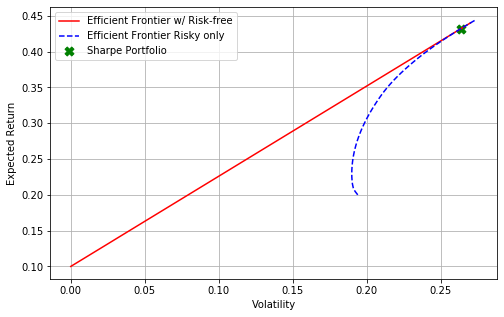
\includegraphics[width=0.7\textwidth]{figures/sharpe_ratio.png}
	\caption{Sharpe portfolio (green cross) compared to the efficient frontier with a risk-free asset (red) and with risky asset only (blue).}
	\label{fig:sharpe_ratio}
\end{figure}

So the optimization using the Sharpe ratio gives us a portfolio that is on the minimum volatility efficient frontier, and gives the maximum return relative to putting all our money in the risk-free asset (so graphically it sits in the tangent point between CAL and efficient frontier).

Usually, any Sharpe ratio greater than 1.0 is considered acceptable to good by investors. A ratio higher than 2.0 is rated as very good. A ratio of 3.0 or higher is considered excellent. A ratio under 1.0 is sub-optimal.

\section{Capital Asset Pricing Model}
\label{sec:capm}
The Capital Asset Pricing Model (CAPM) describes the relationship between expected return of assets and \emph{systematic risk} of the market.

Indeed we can divide a security’s total risk into \emph{unsystematic}, the risk portion peculiar to the company that can be diversified away, and systematic, the nondiversifiable portion that is related to the movement of the stock market and is therefore unavoidable. 

The assumption of CAPM is that investors are risk averse and want to maximize return. This notion implies that investors demand compensation for taking on risk, which in the financial market means that higher-risk securities are priced to yield higher expected returns than lower-risk securities. 

CAPM states that the expected return of an asset is equal to the risk-free return plus a risk premium. 
Mathematically, we can summarize it with the following formula
\begin{equation}
r_i = r_f + \beta_i(r_m-r_f)
\label{eq:capm}
\end{equation}
where:
\begin{itemize}
	\item $r_i$ is the expected return of the $i^{th}$ security;
	\item $r_f$ is the risk-free rate with zero standard deviation (e.g. risk-free asset includes Treasury Bills as they are backed by the U.S. government);
	\item $r_m - r_f$ is the risk premium, $r_m$ denotes the market return including all securities in the market, whose proxy can be an index like SP500;
	\item $\beta_i$ is a measure of $i^{th}$ asset volatility in relation to the overall market. 
	$\beta$ is used in the CAPM to describe the relationship between market risk, and expected return.
\end{itemize}
	
The key point in CAPM is the determination of $\beta$. This can be achieved with the measurement of the slope of the \emph{regression line}, of the market vs individual stock return distribution.

Given two sets of measurements $X$ and $y$ the linear regression determines the parameter $\alpha$ and $\beta$ such that

\begin{equation}
	y=\beta X + \alpha
\end{equation}
by minimizing the sum of the squared differences between the predicted and true $y$ values.
Figure~\ref{fig:linear_regression} shows an example of regression. 
In our case the regressed line estimates the stock returns given the global market returns and in particular 

\begin{equation}
	\beta \approx \cfrac{\textrm{cov}(X,y)}{\textrm {var}(X)}
\end{equation}
so provides insights about how \emph{volatile}, or how risky, a stock is relative to the rest of the market.
In CAPM $\beta$ calculation is used to help investors understand whether a stock moves in the same direction as the rest of the market but for it to provide any useful clue, the market proxy should be related to the stock.

If $\beta$ of an individual stock = 1.0, means its price is perfectly correlated with the market, if $\beta < 1.0$, which is referred to as "defensive", indicates the security is theoretically less volatile than the market (provides lower returns, so it is less risky), while if $\beta > 1.0$, or "aggressive", indicates the assets price is more volatile than the market.

Those who use CAPM pick individual stocks or portfolios, and compare them to different indexes. The point is to find stocks that have high $\beta$, and portfolios that have high $\alpha$. High $\beta$ values mean that the stock fares better than index with positive market and performs worse for negative market (contrary low $\beta$ gives lower performance for positive market and "better" returns in negative market), so those stocks have a chance at beating the market. $\alpha$ values above zero mean that your portfolio outperform market whatever it does.

\begin{figure}[htb]
	\centering
	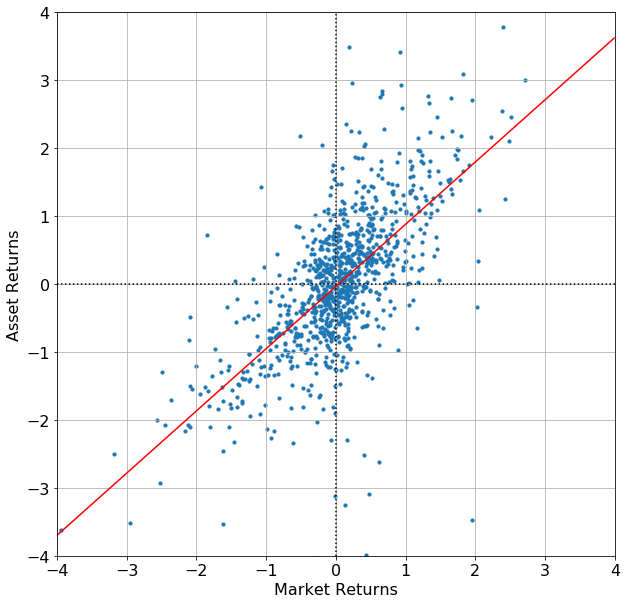
\includegraphics[width=0.7\textwidth]{figures/linear_regression}
	\caption{Example of linear regression for the determination of $\beta$.}
	\label{fig:linear_regression}
\end{figure}

The relationship between risk and expected return is called the \emph{security market line} (SML). An example of this line is shown in Fig.~\ref{fig:sel}. %As indicated before, the expected return on a security generally equals the risk-free rate plus a risk premium. 
In CAPM the risk premium is measured as $\beta$ times the expected return on the market minus the risk-free rate. No measure of unsystematic risk appears in the risk premium, of course, for in the world of CAPM diversification has already eliminated it.

\begin{figure}[htb]
	\centering
	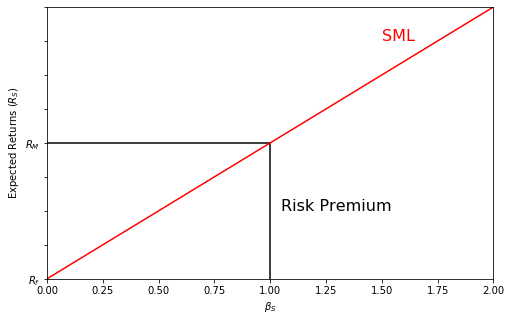
\includegraphics[width=0.7\textwidth]{figures/sel}
	\caption{Security market line.}
	\label{fig:sel}
\end{figure}

In the freely competitive financial markets described by CAPM, no security can sell for long at prices low enough to yield more than its appropriate return on the SML. The security would then be very attractive compared with other securities of similar risk, and investors would bid its price up until its expected return fell to the appropriate position on the SML. Conversely, investors would sell off any stock selling at a price high enough to put its expected return below its appropriate position. The resulting reduction in price would continue until the stock’s expected return rose to the level justified by its systematic risk.

\subsection{Calculate $\beta$ and CAPM for a Stock}

In the following examples historical series of SP500 and some securities are used. They can be gathered with \texttt{ffn}

\begin{ipython}
capm = ffn.get('AAPL,AMZN,BA,GOOG,IBM,MGM,T,TSLA,^GSPC',
               start='2014-03-27', end='2018-03-27')
\end{ipython}
\noindent
or downloaded with \href{https://raw.githubusercontent.com/matteosan1/finance_course/develop/libro/input_files/capm.csv}{capm.csv}.
After an inspection of data, daily and annualized expected returns can be computed.

\begin{ipython}
import pandas as pd

# uncomment this line if using the file
# capm = pd.read_csv("capm.csv", index_col='date')
print (capm.head())
daily_returns = capm.pct_change()*100
\end{ipython}
\begin{ioutput}
                 aapl        amzn          ba        goog         ibm
Date                                                                    
2014-03-27  17.202097  338.470001  105.897987  556.930969  143.243484   
2014-03-28  17.182892  338.290009  106.972359  558.456787  143.711349   
2014-03-31  17.179056  336.369995  107.857635  555.445007  145.250687   
2014-04-01  17.336205  342.989990  110.195465  565.607117  146.767365   
2014-04-02  17.365013  341.959991  110.281410  565.447571  146.050552   

                  mgm          t       tsla         gspc  
Date                                                      
2014-03-27  23.532993  23.542757  41.464001  1849.040039  
2014-03-28  23.514091  23.616835  42.473999  1857.619995  
2014-03-31  24.440292  23.616835  41.689999  1872.339966  
2014-04-01  25.073507  23.630304  43.394001  1885.520020  
2014-04-02  25.234173  23.818861  46.057999  1890.900024  
\end{ioutput}

To recap $\beta$ is the slope of the regression line of the market return vs stock return plot (and $\alpha$ is the intercept of this line with the $y$ axis).

These quantities can be calculated with \texttt{numpy.polyfit} passing as inputs the market and stock return lists. 
The resulting fits for the stocks in our sample are shown in Fig.~\ref{fig:capm_fit}.

With the daily returns and $\beta$ of each stock, we can apply the capital asset pricing model. First, we can calculate the average daily return of the market and this return can be annualized by multiplying it by the number of trading days in a year.
Assuming a risk-free rate of 1\%, we can then calculate CAPM using Eq.~\ref{eq:capm}.

\begin{ipython}
rm = np.mean(daily_returns.iloc[1:]['gspc'])*252
rf = 0.01
betas = {}
alphas = {}
ERs = {}

for i, k in enumerate(df.columns):
    if k == "gspc":
        continue
    betas[k], alphas[k] = np.polyfit(daily_returns['gspc'][1:],
    daily_returns[k][1:], 1)
    ERs[k] = rf + (betas[k] * (rm-rf))

for k, v in ERs.items():
    print ("{:4}: {:4.1f}%".format(k, v))
\end{ipython}
\begin{ioutput}
AAPL: 10.3%
AMZN: 10.8%
BA  : 10.3%
GOOG: 10.7%
IBM :  8.7%
MGM : 13.8%
T   :  5.9%
TSLA: 11.9%
\end{ioutput}

\begin{figure}[htb]
	\centering
	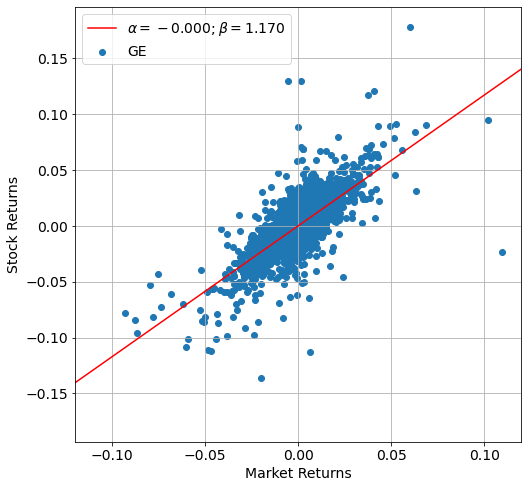
\includegraphics[width=.8\textwidth]{figures/capm_fit.png}
	\caption{Linear regression of market return vs stock return for a set of selected stocks. The fit results are also shown in red and the regression parameters are indicated in the legend.}
	\label{fig:capm_fit}
\end{figure}

\subsection{Calculate $\beta$ and CAPM for a Portfolio}

Now that we have the $\beta$s of each individual stock we can calculate the CAPM for a portfolio made of the same stocks (we assume equal weights for simplicity).
It is enough indeed to perform a weighted sum of of the expected return according to the model of each stock.

\begin{ipython}
print ("{:.1f}%".format(sum(ERs.values())*1/len(ERs)))
\end{ipython}
\begin{ioutput}
10.3%
\end{ioutput}

The expected return of the portfolio is roughly 10\% and this is what an investor should expect according to CAPM.

\subsection{Criticism to CAPM}
As we have seen the whole model is about plotting a line in a scatter plot, it’s not a very complex model. Assumptions under the model are even more simplistic. For example:
\begin{itemize}
\tightlist
\item expect that all investors are rational and they avoid risk;
\item everyone have full information about the market;
\item everyone have similar investment horizons and expectations about future movements;
\item stocks are all correctly priced.
\end{itemize}

Moreover, this is a model from the 1960s. Market dynamics were different back then. And of course, this is a retrospective model. We cannot know how future stock prices move and how the market behaves.
Interesting extension of CAPM involves \emph{Bayesian regression}`\cite{bib:baysean_regression} but it will not be discussed here.

\section{Portfolio Optimization and PCA}
\label{portfolio-optimization-and-pca}

In Section~\ref{sec:pca} the Principal Component Analysis (PCA) has been introduced and here a simple application to portfolio optimization will be described.

Essentially we are going to apply PCA on equity return covariance matrix to construct principal component portfolios because they have some interesting characteristics. This means that our portfolio weights will be based on the eigenvectors of the covariance matrix.

From the theory we know that the first principal component (PC1) is a factor that captures the maximal amount of variance (i.e. the linear combination of assets that has highest possible variance). The second principal component factor (PC2) is the second most variable portfolio that is orthogonal to the first and so on.

It is important to stress that the principal components are just statistical factors that contain no real meaning. However, we will see that the first principal component portfolio is related to the market portfolio (or at least very close to) or to the market risk premium from the CAPM model.

In this analysis we are going to use the equities forming the \emph{Dow Jones 30} index, so the first step is to download their returns with \(\tt{ffn}\) package (the data availability is from March 2019 to today).
	
\begin{ipython}
tickers = ["BA","CAT","CVX","CSCO","KO",
           "DOW","XOM","GS","HD","INTC","IBM",
           "JNJ","JPM","MCD","MRK","MSFT","NKE",
           "PFE","PG","RTX","TRV","UNH","VZ",
           "V","WBA", "WMT", "^DJI"]
           
df = ffn.get(tickers).to_returns().dropna()
\end{ipython}
	
Since the package returns already daily returns we can directly compute the covariance matrix from them. Also we determine eigenvalues and eigenvectors of this matrix.

\begin{ipython}
import numpy as np

equities = df.iloc[:, :-1]
cov = equities.cov()
eigVals, eigVecs = np.linalg.eig(cov)
indices = [i for i in reversed(np.argsort(eigVals))]
l = [eigVals[i]/np.*@sum@*(eigVals)*100 for i in reversed(np.argsort(eigVals))]
\end{ipython}
	
Looking at the plot of the explained variance (see
Fig.~\ref{fig:explained_variance}) we can notice how the first principal
component explains almost 60\% then the value falls quickly down, so we can concentrate only on the first two or three components.

\begin{figure}[htb]
	\centering
	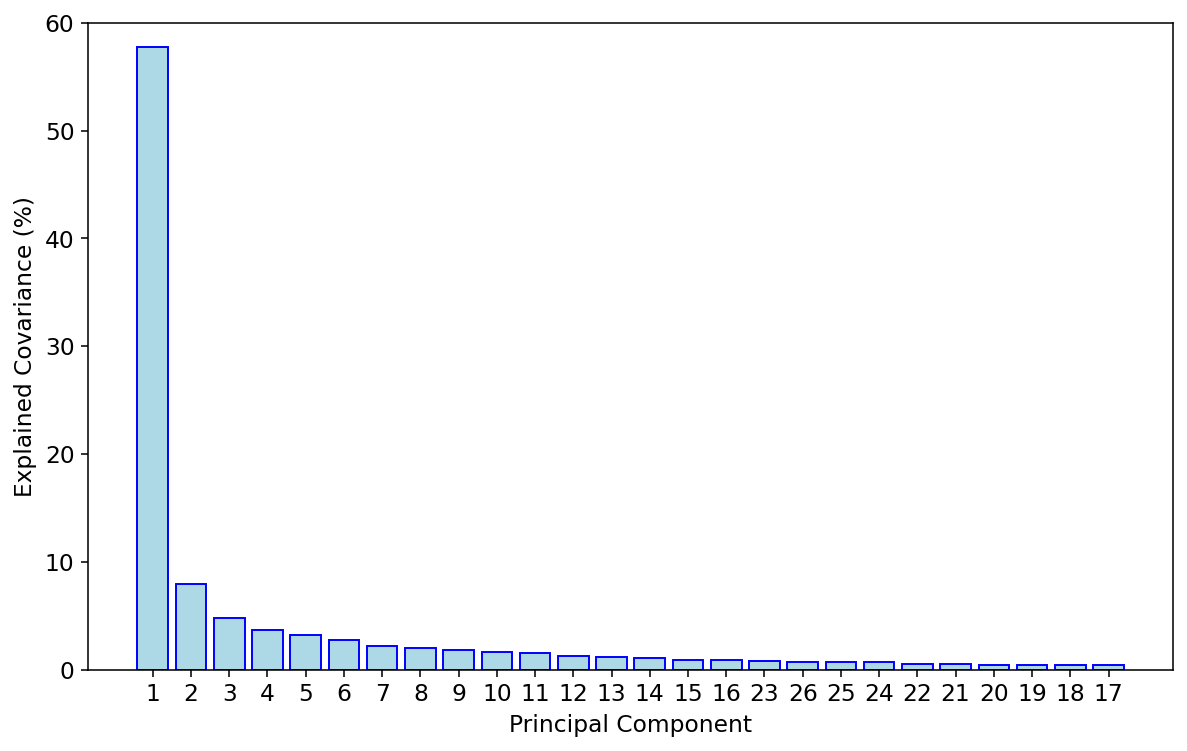
\includegraphics[width=.7\textwidth]{figures/portfolio_pca_expl_var}
	\caption{Explained variance plot. Notice how the explained variance decreases steeply after the first component, and also how the returned components are not ordered by eigenvalue.}
	\label{fig:explained_variance}
\end{figure}
		
Next we can re-scale the PC's eigenvectors to sum up to 1 so they can be
used as portfolio weights.
	
\begin{ipython}
norm_eigVecs = [v/np.linalg.norm(v) for v in eigVecs.T]
\end{ipython}
	
Finally we can construct a portfolio using the weights derived from PCs.
In other words each asset takes a weight equal to its corresponding
component in the PC eigenvector. Figure~\ref{fig:pca_weights} reports
the weights of each asset in PC1 (the first principal component).
	
\begin{figure}[htb]
	\centering
	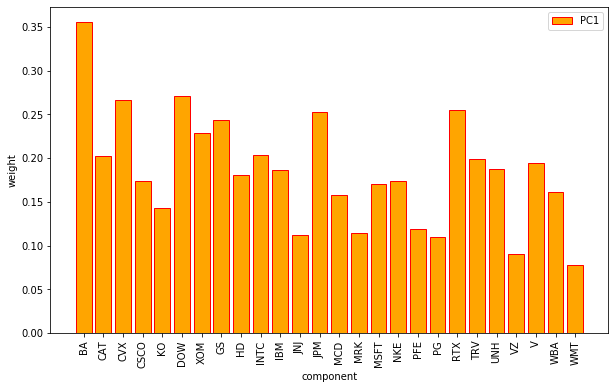
\includegraphics[width=.7\textwidth]{figures/portfolio_pca_pc1_weights}
	\caption{Weights of the PC1 portfolio. Each asset is weighed according
		to the corresponding component in the first principal component
		eigenvector.}
	\label{fig:pca_weights}
\end{figure}
	
Then we calculate the cumulative return of the portfolio and compare the portfolio return to the market return. This process is repeated for the first three components.

\begin{ipython}
for i, index in enumerate(indices[0:3]):
    pc__daily_ret = equities.dot(norm_eigVecs[index])
    pc_cum_ret = pc_daily_ret.cumsum()
    market_cum_ret = df['dji'].cumsum()
\end{ipython}
	
From Fig.~\ref{fig:ret_pc1} to~\ref{fig:ret_pc3} it is clear how the PC1 portfolio return looks identical to the market portfolio. The second and third PC portfolio returns look quite different instead. It is not easy to interpret them, maybe they are connected to higher order momenta. 

\begin{figure}[htb]
	\centering
	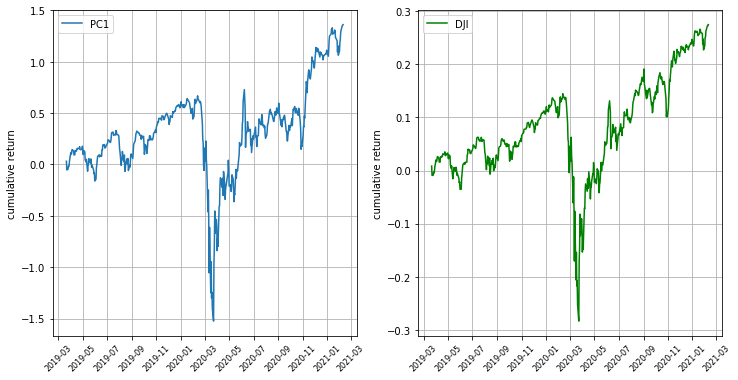
\includegraphics[width=.7\textwidth]{figures/cum_ret_pc1_vs_market}
	\caption{Cumulative return of PC1 portfolio (left) compared to the market return (right).}
	\label{fig:ret_pc1}
\end{figure}

\begin{figure}[htb]
	\centering
	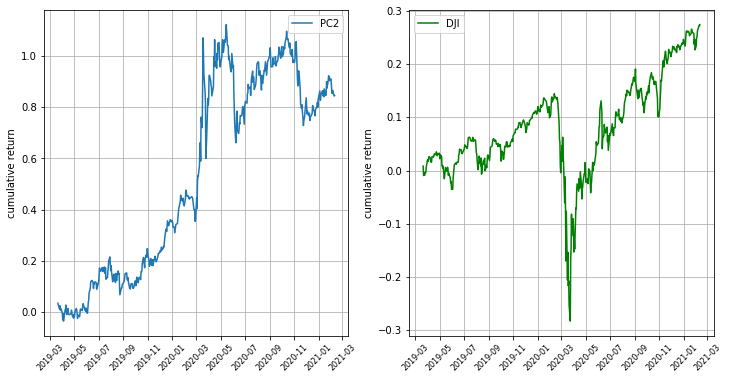
\includegraphics[width=.7\textwidth]{figures/cum_ret_pc2_vs_market}
	\caption{Cumulative return of PC2 portfolio (left) compared to the market return (right).}
	\label{fig:ret_pc2}
\end{figure}

\begin{figure}[htb]
	\centering
	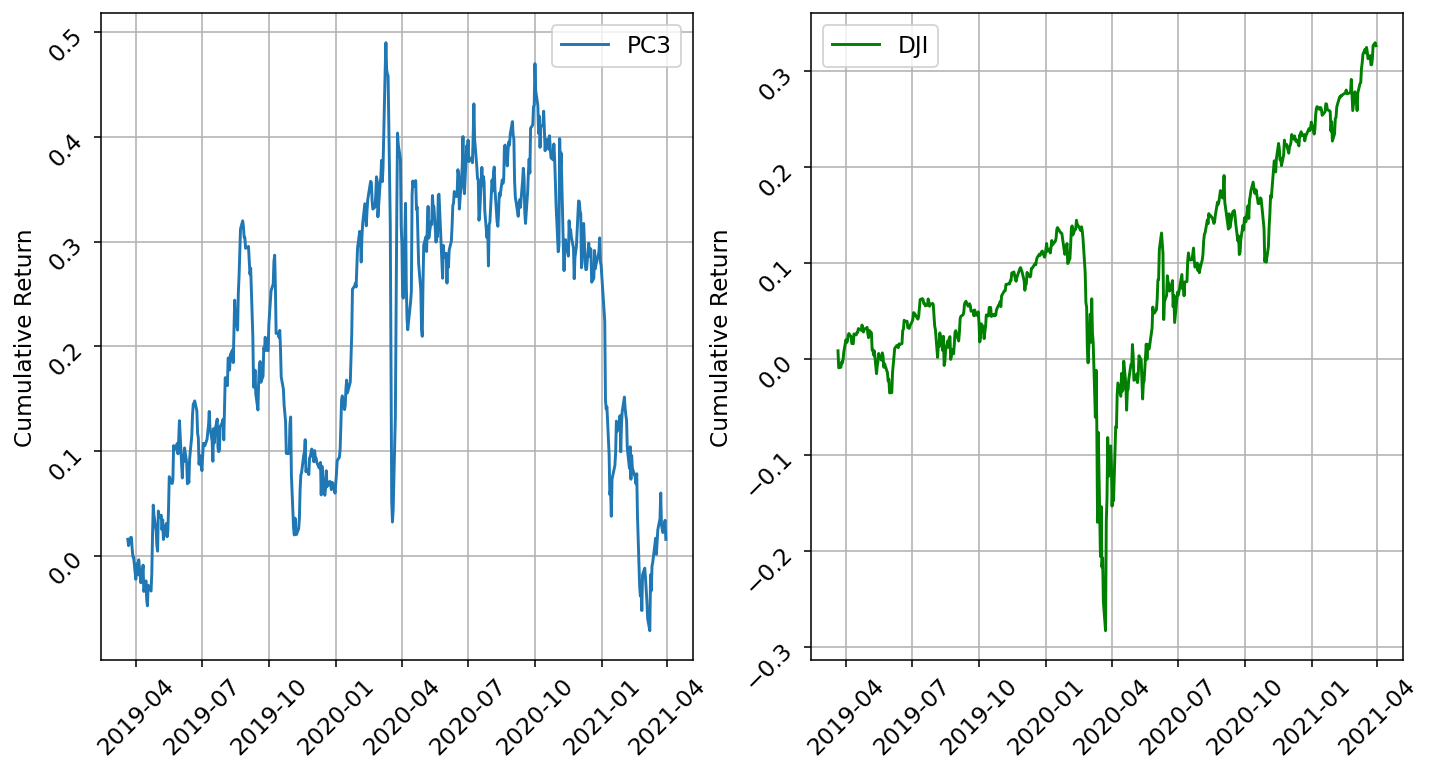
\includegraphics[width=.7\textwidth]{figures/cum_ret_pc3_vs_market}
	\caption{Cumulative return of PC3 portfolio (left) compared to the market return (right).}
	\label{fig:ret_pc3}
\end{figure}

It can be verified that PC1 portfolio
still looks like the market also for other time horizon, repeating the
same steps using weekly or monthly data.

\section{Risk Parity Portfolio}
\label{risk-parity-portfolio}

An alternative approach to Markowitz theory is given by the \emph{risk parity}. A risk parity portfolio is an investment allocation strategy which focuses on the allocation of risk, rather than on the allocation of capital. 
A risk parity (equal risk) portfolio is characterised by having equal risk contributions to the total risk from each individual asset. 

Risk parity allocation is also referred to as equally-weighted risk contributions portfolio method. Equally-weighted risk contributions is not about \emph{having the same volatility}, it is about having each asset contributing in the same way to the portfolio overall volatility. For this we will have to define the contribution of each asset to the portfolio risk. 

This allocation strategy has gained popularity in the last decades since it is believed to provide better risk adjusted return than capital based allocation strategies.

Let's go over a very basic example to better illustrate how to construct a simple risk parity (equal risk) portfolio. Consider a portfolio of \(N\) assets: \(x_{1}, \ldots, x_N\) where as
usual the weight of the $i^{th}$ asset is denoted by \(w_{i}\). The \(w_{i}\) form the allocation vector \(\mathbf{w}\). Let us further denote the covariance matrix of the assets as \(\Sigma\). The volatility of the portfolio is then defined as:

\begin{equation} 
	\sigma_p={\sqrt {\mathbf{w^T}\Sigma \mathbf{w}}} = \sum_{i=1}^{N}\sigma _{i}\qquad\textrm{with}~\sigma _{i} = w_{i}\cdot \cfrac{\partial\sigma_p}{\partial w_{i}}={\cfrac {w_{i}(\Sigma \mathbf{w})_{i}}{\sqrt {\mathbf{w^T}\Sigma \mathbf{w}}}}
\end{equation}
so that \(\sigma _{i}\) can be interpreted as the contribution of the $i^{th}$ asset to the overall risk of the portfolio.

\begin{attention}
\subsubsection{Derivation of $\sigma_i$}
Expressing explicitly in matrix form the standard deviation of the portfolio we get
\[
\begin{split}
	\sigma_p={\sqrt {\mathbf{w^T}\Sigma \mathbf{w}}} & =
	\sqrt{
		\begin{bmatrix}
			w_{1} \\
			w_{2}
		\end{bmatrix}
		\begin{bmatrix}
			\sigma_{11} & \sigma_{21} \\
			\sigma_{12} & \sigma_{22} 
		\end{bmatrix}
		\begin{bmatrix}
			w_{1} & w_{2} \\
		\end{bmatrix}
	}\\
	&=
	\sqrt{
		\begin{bmatrix}
			w_{1} \\
			w_{2}
		\end{bmatrix}
		\begin{bmatrix}
			w_{1}\sigma_{11} + w_{2}\sigma_{12} & w_{1}\sigma_{21} + w_{2}\sigma_{22} \\
		\end{bmatrix}
	} \\
	&= \sqrt{
		w_{1}w_{1}\sigma_{11} + w_{2}w_{1}\sigma_{12} + w_{1}w_{2}\sigma_{21} + w_{2}w_{2}\sigma_{22} }
\end{split}
\]
Now performing for example the derivative with respect to $w_1$ we obtain
\[\cfrac{\partial\sigma_p}{\partial w_1} = \cfrac{1}{2}\cdot\cfrac{2\cdot w_1\sigma_{11} + 2\cdot w_{2}\sigma_{21}}{\sigma_p} = \cfrac{w_1\sigma_{11} + w_{2}\sigma_{21}}{\sigma_p} = \cfrac{(\Sigma \mathbf{w})_{1}}{\sigma_p}\]

Summing up $\sum w_i\cdot\cfrac{\partial\sigma_p}{\partial w_i}$ we get back $\sigma_p$
\end{attention}

Equal risk contribution then means \(\sigma _{i} =\sigma _{j}\) for all \(i,j\) or equivalently \(\sigma _{i}=\sigma_p/N\). So

\begin{equation}
\sigma _{i} = \cfrac{\sigma_p}{N}={\cfrac {w_{i}(\Sigma \mathbf{w})_{i}}{\sqrt {\mathbf{w^T}\Sigma \mathbf{w}}}}\implies w_{i} = \frac {\sigma_p^{2}}{(\Sigma \mathbf{w})_{i}N}
\end{equation}
Since we want the previous expression to be true for each $i$, the solution for the weights can be found by solving the minimisation problem

\begin{equation} 
\underset{\mathbf{w}}{\min } \sum _{i=1}^{N}\left[w_{i}-{\frac {\sigma_p^{2}}{(\Sigma \mathbf{w})_{i}N}}\right]^{2} 
\end{equation}

Going back to our data sample let's find out the weights to give us a risk parity portfolio.

\begin{ipython}
num_assets = 5
def risk_parity(w, cov):
    variance = w.T.dot(cov.dot(w))
    sum = 0
    N = len(w)
    for i in range(N):
        sum += (w[i] - (variance/(N*cov.dot(w)[i])))**2
    return sum

args = (covariance,)
constraints = ({'type': 'eq', 'fun': sum_weights})
bounds = tuple((0, 1) for asset in range(num_assets))
weights = [1./num_assets for _ in range(num_assets)]
opts = minimize(risk_parity, weights, args=(covariance,),
                bounds=bounds, constraints=constraints)
print (opts)
\end{ipython}
\begin{ioutput}
    fun: 2.2881862766486147e-07
    jac: array([-6.98851511e-04,  1.92391042e-04, -4.08403758e-05, 
                -2.54432521e-05,  1.13250609e-03])
message: 'Optimization terminated successfully.'
   nfev: 38
    nit: 5
   njev: 5
 status: 0
success: True
      x: array([0.25863039, 0.18154282, 0.19666705, 0.22190633, 
                0.14125342])
\end{ioutput}

\begin{ipython}
sigma_i = []
std = np.sqrt(opts.x.T.dot(covariance.dot(opts.x)))
for i in range(num_assets):
    a = opts.x[i]*covariance.dot(opts.x)[i]
    sigma_i.append(a/std)

for i in range(num_assets):
    print ("Risk contribution for asset {}: {:.3f}%"
           .format(i, sigma_i[i]/sum(sigma_i)*100))
\end{ipython}
\begin{ioutput}
Risk contribution for asset 0: 19.974%
Risk contribution for asset 1: 19.999%
Risk contribution for asset 2: 19.990%
Risk contribution for asset 3: 19.992%
Risk contribution for asset 4: 20.045%
\end{ioutput}

%Figure~\ref{fig:risk_parity} shows the fraction of risk allocated to each asset and the corresponding weight within the portfolio.

\subsection{Risk Budget Allocation}
\label{risk-budget-allocation}

The same technique can be used if we would like to calculate a portfolio
with risk budget allocation. In this case we want to associate to each asset a particular level of risk. If we consider the previous equation

\begin{equation} 
\sigma _{i}=\cfrac{\sigma_p}{N} 
\end{equation}
where we set the risk contribution fraction to every asset to \(1/N\);
now we can simply replace \(1/N\) with the desired fraction of risk (\(f_i\)) for each asset

\begin{equation} 
\sigma _{i}=f_i \cdot \sigma_p 
\end{equation}
so that the relation to minimise becomes

\begin{equation} 
\underset{\mathbf{w}}{\min} \sum _{i=1}^{N}\left[w_{i}-{\frac {f_i \cdot \sigma_p^{2}}{(\Sigma \mathbf{w})_{i}}}\right]^{2} 
\end{equation}

Translating it into \texttt{python} we get:

\begin{ipython}
def risk_budget(w, target_risk, cov):
    variance = w.T.dot(cov.dot(w))
    sum = 0
    N = len(w)
    for i in range(N):
        sum += (w[i] - (target_risk[i]*variance)/(cov.dot(w)[i]))**2
    return sum

f_i = [0.3, 0.2, 0.2, 0.15, 0.15]
args = (f_i, covariance)
constraints = ({'type': 'eq', 'fun': sum_weights})
bounds = tuple((0, 1) for asset in range(num_assets))
weights = [1./num_assets for _ in range(num_assets)]
opts = minimize(risk_budget, weights, args=(f_i, covariance),
                bounds=bounds, constraints=constraints)
print (opts)
\end{ipython}
\begin{ioutput}
    fun: 4.058673684147486e-08
    jac: array([-2.64817707e-04,  3.30937403e-04,  2.14530647e-05, 
                -7.65372775e-05,  3.67853561e-04])
message: 'Optimization terminated successfully.'
   nfev: 45
    nit: 6
   njev: 6
 status: 0
success: True
      x: array([0.3459366 , 0.1800917 , 0.19394454, 0.16890483, 
                0.11112233])
\end{ioutput}
\begin{ipython}  
sigma_i = []
std = np.sqrt(opts.x.T.dot(covariance.dot(opts.x)))
for i in range(num_assets):
    a = opts.x[i]*covariance.dot(opts.x)[i]
    sigma_i.append(a/std)

for i in range(num_assets):
    print ("Risk contribution for asset {}: {:.3f}%"
           .format(i, sigma_i[i]/sum(sigma_i)*100))    
\end{ipython}
\begin{ioutput}
Risk contribution for asset 0: 29.988%
Risk contribution for asset 1: 20.010%
Risk contribution for asset 2: 19.996%
Risk contribution for asset 3: 14.993%
Risk contribution for asset 4: 15.012%
\end{ioutput}

%Figure~\ref{risk_allocation} shows the amount of risk associated to each asset and their weights within the portfolio. 
Indeed for each stock we have allocated the desired amount of risk.

\section{Portfolio Diversification}

Diversification is a common topic in portfolio construction and allows to combine risky stocks so that their combination (the portfolio) is less risky than any of its components. Although such diversification is a familiar notion, it may be worthwhile to review the manner in which diversification reduces risk.

Suppose there are two companies located on an isolated island whose chief industry is tourism. One company manufactures suntan lotion. Its stock predictably performs well in sunny years and poorly in rainy ones. The other company produces umbrellas. Its stock performs equally poorly in sunny years and well in rainy ones. Each company earns a 12\% average return.

In purchasing either stock, investors incur a great amount of risk because of variability in the stock price driven by fluctuations in weather conditions. Investing half the funds in the suntan lotion stock and half in the stock of the umbrella manufacturer, however, results in a return of 12\% regardless of which weather condition prevails. Portfolio diversification thus transforms two risky stocks, each with an average return of 12\%, into a riskless portfolio certain of earning the expected 12\%.

Unfortunately, the perfect negative relationship between the returns on these two stocks is very rare in the real world. To some extent, corporate securities move together, so complete elimination of risk through simple portfolio diversification is impossible. However, as long as some lack of parallelism in the returns of securities exists, diversification will always reduce risk.

Empirical studies have demonstrated that unsystematic risk can be virtually eliminated in portfolios of 30 to 40 randomly selected stocks. Of course, if investments are made in closely related industries, more securities are required to eradicate it.

As we have already seen no measure of unsystematic risk appears in the risk premium, of CAPM model, since it is assumed that diversification has eliminated it.

In the Markowitz model instead diversification is achieved by seeking to combine in a portfolio assets with returns that are less than perfectly positively correlated, in an effort to lower portfolio risk (variance) without sacrificing return, through the reduction of the correlation matrix $\Sigma$.

\subsection{Maximum Diversification Portfolio}
\label{maximum-diversification-portfolio}

Diversification it is most often either pursued in tandem with another objective, such as return maximization, or pursued simply by including more asset classes or adding constraints based on intuition.

But it does not have to be this way and diversification can be pursued explicitly as the sole objective in portfolio construction.
In a 2008 paper~\cite{bib:diversification}, the diversification ratio $D$ of a portfolio has been defined as

\begin{equation}
D=\cfrac{\mathbf{w^T}\boldsymbol{\sigma}}{\sqrt {\mathbf{w^T}\Sigma \mathbf{w}}} 
\end{equation}
where $\boldsymbol{\sigma}$ is the vector of volatilities and $\Sigma$ is the covariance matrix. The denominator represents the volatility of the portfolio and the numerator the weighted average volatility of the assets. More diversification within a portfolio decreases the denominator and leads to a higher diversification ratio.
Let's construct a portfolio that maximize this ratio.

\begin{ipython}
def diversification_ratio(w):
    w_vol = np.dot(np.sqrt(np.diag(covariance)), w.T)
    port_vol = np.sqrt(np.dot(w.T, np.dot(covariance, w)))
    diversification_ratio = w_vol/port_vol
    return -diversification_ratio

bounds = tuple((0, 1) for asset in range(num_assets))
cons = ({'type': 'eq', 'fun': sum_weights},)
#cons = cons + ({'type': 'ineq', 'fun': long_only_constraint},)
weights = [1./num_assets for _ in range(num_assets)]
opts = minimize(diversification_ratio, weights, bounds=bounds,
                constraints=cons)
print (opts)
\end{ipython}
\begin{ioutput}
    fun: -1.3580745811820554
    jac: array([-0.00035974,  0.00029349, -0.00035594,  0.00077944,  
                 0.00016446])
message: 'Optimization terminated successfully.'
   nfev: 36
    nit: 5
   njev: 5
 status: 0
success: True
      x: array([0.34867985, 0.18062199, 0.15557008, 0.1235694, 
                0.19155868])
\end{ioutput}
\begin{ipython}
ret = np.*@sum@*(returns*opts.x)
vol = np.sqrt(np.dot(opts.x.T, np.dot(covariance, opts.x)))
print ("Diversification: ", -opts.fun)
\end{ipython}
\begin{ioutput}
Diversification: 1.3580745811820554
\end{ioutput}

Figure~\ref{fig:max_div} shows how the maximum diversified portfolio compares to the efficient frontier.

\begin{figure}[htb]
	\centering
	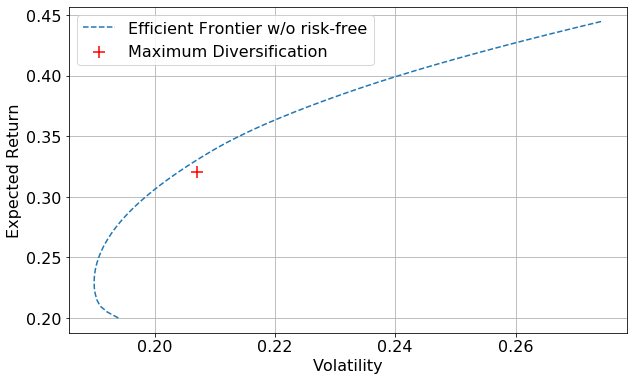
\includegraphics[width=0.7\textwidth]{figures/max_div.png}
	\caption{Portfolio constructed with the maximum diversification technique shown in the return/variance plane.}
	\label{fig:max_div}
\end{figure}

\section{Exercises}
\begin{question}
One of the approaches to finding the optimal point on the efficient frontier for a given investor is to maximize the investor's utility ($U$). This is a measure of how much benefit investors obtain from portfolio performance. Utility is a measure of relative satisfaction that an investor derives from different portfolios. Utility is a function of the portfolio expected return, the portfolio variance and a measure of risk aversion

\begin{equation*}
U = \mathbb{E}(R_{p}) - \frac{1}{2}A\sigma^2
\end{equation*}
where $U$ = utility, $\mathbb{E}(R)$ = portfolio expected return, $A$ = risk aversion coefficient and $\sigma^2$ = portfolio variance.
In determining the risk aversion ($A$), we measure the marginal reward an investor needs in order to take on more risk. A risk-averse investor will need a high margin reward for taking on more risk. The utility equation shows the following:
\begin{itemize}
\tightlist
\item $U$ can be positive or negative, i.e. it is unbounded;
\item high returns add to utility;
\item high variance reduces utility;
\item $U$ does not measure satisfaction but can be used to rank portfolios.
\end{itemize}

The risk aversion coefficient, $A$, ranges between 1 and 10 (1 for the aggressive investor, 4 for the moderate investor, and 10 for the risk-averse investor.

Given the historical series in \href{https://github.com/matteosan1/finance_course/raw/master/input_files/share_price.csv}{share\_prices.csv} find the best portfolio for aggressive, moderate and risk-averse investors.

\end{question}

\cprotEnv \begin{solution}
\begin{ipython}
import pandas as pd
df = pd.read_csv("share_prices.csv", index_col='Date')
daily_returns = df.pct_change()
returns = daily_returns.mean()*252
covariance = daily_returns.cov()*252

print (returns)
print (covariance)
\end{ipython}
\begin{ioutput}
CHD     0.062666
COST    0.247429
CTRE    0.165151
ENTR    0.002445
HI      0.223906
LDOS    0.075464
TDS    -0.003953
TMUS    0.283815
UEC     0.999521
WM      0.163298
dtype: float64

           CHD     COST       CTRE      ENTR        HI      LDOS       TDS
CHD   0.067815  0.036114  0.016454  0.022583  0.022301  0.029738  0.032921   
COST  0.036114  0.073004  0.031599  0.049279  0.034606  0.034481  0.034043   
CTRE  0.016454  0.031599  0.313706  0.074262  0.136719  0.068927  0.088424   
ENTR  0.022583  0.049279  0.074262  0.113892  0.062266  0.043155  0.040843   
HI    0.022301  0.034606  0.136719  0.062266  0.202751  0.068284  0.097420   
LDOS  0.029738  0.034481  0.068927  0.043155  0.068284  0.110635  0.059296   
TDS   0.032921  0.034043  0.088424  0.040843  0.097420  0.059296  0.185842   
TMUS  0.026069  0.042121  0.073199  0.055806  0.057519  0.046704  0.068516   
UEC   0.045100  0.099269  0.164647  0.147985  0.165341  0.096700  0.143037   
WM    0.034987  0.034676  0.049294  0.034555  0.057760  0.047310  0.048338   
...
\end{ioutput}
\begin{ipython}
import numpy as np
from scipy.optimize import minimize

def sum_weights(w): 
    return np.sum(w) - 1

def utility(w, returns, cov, risk_aversion):
    return -(returns.dot(w) - 0.5*w.T.dot(cov.dot(w))*risk_aversion)

num_assets = 10
constraints = [{'type': 'eq', 'fun': sum_weights},] 
bounds = tuple((0, 1) for _ in range(num_assets))
weights = [1./num_assets for _ in range(num_assets)]

for risk_aversion in (1, 4, 10):
  opts = minimize(utility, weights, args=(returns, covariance, risk_aversion),
                bounds=bounds, constraints=constraints)
  for i, c in enumerate(df.columns):
    print ("{} {:.1f}".format(c, opts.x[i]*100), end=" ")
  print()
  print ("Expected return: {:.3f}".format(opts.x.dot(returns)))
  print ("Variance: {:.3f}".format(opts.x.T.dot(covariance.dot(opts.x))))
\end{ipython}
\begin{ioutput}
# aggressive
CHD 0.0 COST 0.0 CTRE 0.0 ENTR 0.0 HI 0.0 LDOS 0.0 TDS 0.0 TMUS 12.8 UEC 87.2 WM 0.0 
Expected return: 0.908
Variance: 0.734

# moderate
CHD 0.0 COST 47.2 CTRE 0.0 ENTR 0.0 HI 0.0 LDOS 0.0 TDS 0.0 TMUS 33.1 UEC 18.3 WM 1.4 
Expected return: 0.396
Variance: 0.104

# risk averse
CHD 7.1 COST 40.2 CTRE 0.0 ENTR 0.0 HI 1.3 LDOS 0.0 TDS 0.0 TMUS 22.7 UEC 4.1 WM 24.6 
Expected return: 0.252
Variance: 0.055
\end{ioutput}
\end{solution}

\begin{question}
Your are portfolio manager and one of your clients is asking to design her investment in order to reduce at the minimum the risk. Her position involves these shares: 'TMUS', 'TDS', 'ENTR', 'UEC', 'WM', 'CTRE', 'LDOS', 'COST', 'CHD', 'HI'.
Find the weights corresponding to each asset.

\noindent\textbf{Hint:} the historical series of the corresponding companies are stored in \href{https://github.com/matteosan1/finance_course/raw/master/input_files/share_price.csv}{share\_prices.csv}.

\end{question}

\cprotEnv \begin{solution}
\begin{ipython}
import pandas as pd
df = pd.read_csv("share_prices.csv", index_col='Date')

daily_returns = df.pct_change()
returns = daily_returns.mean()*252
covariance = daily_returns.cov()*252
\end{ipython}
\begin{ipython}
import numpy as np
from scipy.optimize import minimize

def sum_weights(w):
    return np.sum(w) - 1

def min_risk(w, cov):
    return np.sqrt(w.T.dot(cov.dot(w)))

num_assets = 10
constraints = ({'type': 'eq', 'fun': sum_weights},)
bounds = tuple((0, 1) for asset in range(num_assets))
weights = [1./num_assets for _ in range(num_assets)]
opts = minimize(min_risk, weights, args=(covariance,),
                bounds=bounds, constraints=constraints)

print (opts)
\end{ipython}
\begin{ioutput}
     fun: 0.20887087318996655
     jac: array([0.2088003 , 0.20897953, 0.20895358, 0.20911743, 0.21106115,
                 0.20858843, 0.20914311, 0.20901022, 0.40519709, 0.20881298])
 message: 'Optimization terminated successfully'
    nfev: 110
     nit: 10
    njev: 10
  status: 0
 success: True
       x: array([3.33744344e-01, 1.68530140e-01, 8.18977235e-03, 9.91808728e-02,
                 0.00000000e+00, 7.10377889e-02, 6.05724516e-03, 8.44657341e-02,
                 3.89635156e-20, 2.28794102e-01])
\end{ioutput}
\begin{ipython}
print ("Portfolio composition")
for i, n in enumerate(df.columns):
    print ("{:5}: {:4.1f}%".format(n, opts.x[i]*100))
print ("Portfolio variance: {:.4f}".format(opts.fun**2))
print ("Expected Portfolio return: {:.3f}".format(opts.x.dot(returns)))
\end{ipython}
\begin{ioutput}
Portfolio composition
CHD  : 33.4%
COST : 16.9%
CTRE :  0.8%
ENTR :  9.9%
HI   :  0.0%
LDOS :  7.1%
TDS  :  0.6%
TMUS :  8.4%
UEC  :  0.0%
WM   : 22.9%
Portfolio variance: 0.0436
Expected Portfolio return: 0.131
\end{ioutput}
\end{solution}

%\begin{question}[title={(Return Allocation Portfolio)}]
%After few months the same client of the previous question, contacted you again asking for larger returns. In particular she would like to increase it by 40\%.
%Find the new portfolio composition that makes your client happy.
%\end{question}
%\begin{solution}
%\begin{tcolorbox}[size=fbox, boxrule=1pt, colback=cellbackground, colframe=cellborder]
%\begin{Verbatim}[commandchars=\\\{\}]
%\PY{k}{def} \PY{n+nf}{efficient\PYZus{}frontier}\PY{p}{(}\PY{n}{w}\PY{p}{,} \PY{n}{asset\PYZus{}returns}\PY{p}{,} \PY{n}{target\PYZus{}return}\PY{p}{)}\PY{p}{:} 
%    \PY{n}{portfolio\PYZus{}return} \PY{o}{=} \PY{n}{np}\PY{o}{.}\PY{n}{sum}\PY{p}{(}\PY{n}{asset\PYZus{}returns} \PY{o}{*} \PY{n}{w}\PY{p}{)} 
%    \PY{k}{return} \PY{p}{(}\PY{n}{portfolio\PYZus{}return} \PY{o}{\PYZhy{}} \PY{n}{target\PYZus{}return}\PY{p}{)}
%		
%\PY{n}{results} \PY{o}{=} \PY{p}{[}\PY{p}{]}
%\PY{n}{bounds} \PY{o}{=} \PY{n+nb}{tuple}\PY{p}{(}\PY{p}{(}\PY{l+m+mi}{0}\PY{p}{,} \PY{l+m+mi}{1}\PY{p}{)} \PY{k}{for} \PY{n}{asset} \PY{o+ow}{in} \PY{n+nb}{range}\PY{p}{(}\PY{n}{num\PYZus{}assets}\PY{p}{)}\PY{p}{)}
%\PY{n}{target} \PY{o}{=} \PY{l+m+mf}{0.172}\PY{o}{*}\PY{l+m+mf}{1.4}
%\PY{n}{constraints} \PY{o}{=} \PY{p}{(}\PY{p}{\PYZob{}}\PY{l+s+s1}{\PYZsq{}}\PY{l+s+s1}{type}\PY{l+s+s1}{\PYZsq{}}\PY{p}{:} \PY{l+s+s1}{\PYZsq{}}\PY{l+s+s1}{eq}\PY{l+s+s1}{\PYZsq{}}\PY{p}{,} \PY{l+s+s1}{\PYZsq{}}\PY{l+s+s1}{fun}\PY{l+s+s1}{\PYZsq{}}\PY{p}{:} \PY{n}{efficient\PYZus{}frontier}\PY{p}{,} 
%                \PY{l+s+s1}{\PYZsq{}}\PY{l+s+s1}{args}\PY{l+s+s1}{\PYZsq{}}\PY{p}{:}\PY{p}{(}\PY{n}{returns}\PY{p}{,} \PY{n}{target}\PY{p}{)}\PY{p}{\PYZcb{}}\PY{p}{,}
%               \PY{p}{\PYZob{}}\PY{l+s+s1}{\PYZsq{}}\PY{l+s+s1}{type}\PY{l+s+s1}{\PYZsq{}}\PY{p}{:} \PY{l+s+s1}{\PYZsq{}}\PY{l+s+s1}{eq}\PY{l+s+s1}{\PYZsq{}}\PY{p}{,} \PY{l+s+s1}{\PYZsq{}}\PY{l+s+s1}{fun}\PY{l+s+s1}{\PYZsq{}}\PY{p}{:} \PY{n}{sum\PYZus{}weights}\PY{p}{\PYZcb{}}\PY{p}{)}
%\PY{n}{weights} \PY{o}{=} \PY{p}{[}\PY{l+m+mf}{1.}\PY{o}{/}\PY{n}{num\PYZus{}assets} \PY{k}{for} \PY{n}{\PYZus{}} \PY{o+ow}{in} \PY{n+nb}{range}\PY{p}{(}\PY{n}{num\PYZus{}assets}\PY{p}{)}\PY{p}{]}
%\PY{n}{opts} \PY{o}{=} \PY{n}{minimize}\PY{p}{(}\PY{n}{markowitz}\PY{p}{,} \PY{n}{weights}\PY{p}{,} \PY{n}{args}\PY{o}{=}\PY{p}{(}\PY{n}{covariance}\PY{p}{,}\PY{p}{)}\PY{p}{,}
%\PY{n}{bounds}\PY{o}{=}\PY{n}{bounds}\PY{p}{,} \PY{n}{constraints}\PY{o}{=}\PY{n}{constraints}\PY{p}{)} 
%		
%\PY{n}{p\PYZus{}variance} \PY{o}{=} \PY{n}{np}\PY{o}{.}\PY{n}{dot}\PY{p}{(}\PY{n}{opts}\PY{o}{.}\PY{n}{x}\PY{o}{.}\PY{n}{T}\PY{p}{,} \PY{n}{np}\PY{o}{.}\PY{n}{dot}\PY{p}{(}\PY{n}{covariance}\PY{p}{,} \PY{n}{opts}\PY{o}{.}\PY{n}{x}\PY{p}{)}\PY{p}{)}
%\PY{n}{ret} \PY{o}{=} \PY{n}{np}\PY{o}{.}\PY{n}{sum}\PY{p}{(}\PY{n}{returns}\PY{o}{*}\PY{n}{opts}\PY{o}{.}\PY{n}{x}\PY{p}{)}
%\PY{n+nb}{print} \PY{p}{(}\PY{l+s+s2}{\PYZdq{}}\PY{l+s+s2}{Portfolio variance: }\PY{l+s+si}{\PYZob{}:.3f\PYZcb{}}\PY{l+s+s2}{\PYZdq{}}\PY{o}{.}\PY{n}{format}\PY{p}{(}\PY{n}{variance}\PY{p}{)}\PY{p}{)}
%\PY{n+nb}{print} \PY{p}{(}\PY{l+s+s2}{\PYZdq{}}\PY{l+s+s2}{Portfolio return: }\PY{l+s+si}{\PYZob{}:.3f\PYZcb{}}\PY{l+s+s2}{\PYZdq{}}\PY{o}{.}\PY{n}{format}\PY{p}{(}\PY{n}{ret}\PY{p}{)}\PY{p}{)}
%
%Portfolio variance: 0.026
%Portfolio return: 0.241
%\end{Verbatim}
%\end{tcolorbox}	
%\end{solution}

\begin{question}
The client is not yet satisfied and decides to move to a risk parity portfolio. Compute the correct weights to have each asset contributing equally to the portfolio risk.
\end{question}

\cprotEnv \begin{solution}
\begin{ipython}
def risk_parity(w, cov):
    variance = w.T.dot(cov.dot(w))
    sum = 0 
    N = len(w)
    for i in range(N):
        sum += (w[i] - (variance/(N*(cov.dot(w))[i])))**2
    return sum

args = (covariance,)
constraints = ({'type': 'eq', 'fun': sum_weights})
bounds = tuple((0, 1) for asset in range(num_assets))
weights = [1./num_assets for _ in range(num_assets)]
opts = minimize(risk_parity, weights, args=(covariance,),
                bounds=bounds, constraints=constraints)

print (opts)
\end{ipython}
\begin{ioutput}
     fun: 3.5766519241779855e-07
     jac: array([ 1.24834913e-03,  1.00388202e-03, -2.28052647e-04,  6.19051279e-04,
                 -5.68149005e-04, -1.03169022e-03, -1.24285291e-03, -4.09550915e-04,
                 -2.02491654e-03,  6.26250036e-06])
 message: 'Optimization terminated successfully'
    nfev: 80
     nit: 7
    njev: 7
  status: 0
 success: True
       x: array([0.161952  , 0.12997992, 0.07022277, 0.10331577, 0.07717795,
                 0.10490077, 0.08475445, 0.10276264, 0.04079525, 0.12413849])
\end{ioutput}
\begin{ipython}
sigma_i = []
for i in range(num_assets):
    std = np.sqrt(opts.x.T.dot(covariance.dot(opts.x)))
    a = opts.x[i]*covariance.dot(opts.x)[i]
    sigma_i.append(a/std)

for i in range(num_assets):
    print ("Risk contribution for asset {}: {:6.3f}%"
           .format(i, sigma_i[i]/sum(sigma_i)*100))
\end{ipython}
\begin{ioutput}
Risk contribution for asset 0:  9.986%
Risk contribution for asset 1: 10.003%
Risk contribution for asset 2:  9.971%
Risk contribution for asset 3:  9.987%
Risk contribution for asset 4: 10.014%
Risk contribution for asset 5:  9.998%
Risk contribution for asset 6: 10.047%
Risk contribution for asset 7:  9.976%
Risk contribution for asset 8: 10.023%
Risk contribution for asset 9:  9.995%		
\end{ioutput}
\end{solution}



\begin{thebibliography}{9}
\bibitem{bib:post_modern_theory}\href{https://en.wikipedia.org/wiki/Post-modern_portfolio_theory}{\emph{Post Modern Theory}}, Wikipedia [Online]
\bibitem{bib:black_litterman}\href{https://en.wikipedia.org/wiki/Black\%E2\%80\%93Litterman_model}{\emph{Black-Litterman Model}}, Wikipedia [Online]
\bibitem{bib:bayesian_regression}W. Kohersen, \href{https://towardsdatascience.com/introduction-to-bayesian-linear-regression-e66e60791ea7}{\emph{Introduction to Bayesian Linear Regression}}, Toward Data Science [Online]
\bibitem{bib:diversification} Y. Choueifaty, Y.Coignard, \href{ https://www.tobam.fr/wp-content/uploads/2014/12/TOBAM-JoPM-Maximum-Div-2008.pdf}{\emph{Toward Maximum Diversification}}, 2008
\end{thebibliography}